\documentclass[openany,a4paper,12pt]{article}
%%%%%%%%%%%%%%%%%%%%%%%%%%%%%%%  * PACKAGES *  %%%%%%%%%%%%%%%%%%%%%%%%%%%%%%%%%%%%

%% DOC   --------------------------------------------------------------------------

\usepackage[utf8]{inputenc}
\usepackage[english,french]{babel}
\usepackage[top=3cm, bottom=3cm, left=3cm, right=3cm]{geometry}
%\usepackage{charter}
%\usepackage{fancyhdr}
%\usepackage{lastpage}

%% FONTS ET SPACES   --------------------------------------------------------------

%\usepackage{setspace}
%\onehalfspacing

%\usepackage{times}
%\usepackage{fontspec}
%\setmainfont{Times}
%\fontsize{12pt}
%\fontfamily{ptm}

%\usepackage{libertine}
%\usepackage{biolinum}
%\usepackage{libertinust1math}
%\usepackage[T1]{fontenc}

%% OTHER PACKAGES   ---------------------------------------------------------------

\usepackage{physics}
%\usepackage{chemformula}
%\usepackage{algorithmicx}
%\usepackage{pythonhighlight}

\usepackage{amsmath}
\usepackage{amssymb}
%\usepackage{amsthm}
%\numberwithin{equation}{section}
\usepackage{siunitx}
%\usepackage[squaren,Gray]{SIunits}

\usepackage{wrapfig}
\usepackage{graphicx}
%\usepackage{booktabs}
%\usepackage{framed}

%\usepackage{environ}
%\usepackage{tikz}
%\usetikzlibrary{decorations.pathmorphing,patterns}
%\usetikzlibrary{calc}
%\usepackage{pgfplots}
%\usepgfplotslibrary{fillbetween}

\usepackage{caption}
\usepackage{subcaption} % two figures side by side
%\usepackage{longtable} % needed for long tables over pages
%\usepackage{enumerate} % needed for some options in enumerate

\usepackage{hyperref}
\usepackage{todonotes} % needed for todos
%\usepackage{tocloft} 
%\usepackage{makeidx} % needed for creating an index
%\makeindex

%\usepackage{listings}

%% LINKS   ------------------------------------------------------------------------

%\usepackage[hidelinks=true,colorlinks=true
%,breaklinks]{hyperref}
%\usepackage{xcolor}
%\definecolor{c1}{rgb}{0,0,1} % blue
%\definecolor{c2}{rgb}{0,0.25,0.75} % green blue
%\definecolor{c3}{rgb}{0.25,0,0.75} % red blue
%\hypersetup{
%	linkcolor={c1}, % internal links
%	citecolor={c1}, % citations
%	urlcolor={c3}, % external links/urls
%	runcolor={c1} % executable links
%}
%\usepackage[hyphenbreaks]{breakurl}


%% BIBLIOGRAPHY
%% BIBLIOGRAPHY   -----------------------------------------------------------------

\usepackage[hyperref=true,
url=true,
isbn=false,
backref=true,
style=custom-numeric-comp,
citereset=section,
maxcitenames=3,
maxbibnames=100,
backend=bibtex, % while checking on one of my (newest) systems, this option was needed to generate bibliography
block=none]{biblatex}

% back reference text preceding the page number ("see p.")
\DefineBibliographyStrings{english}{%
	backrefpage  = {see p.}, % for single page number
	backrefpages = {see pp.} % for multiple page numbers
}

% the followings activate 'custom-english-ordinal-sscript.lbx'
% in order to print ordinal 'edition' suffixes as superscripts,
% and adjusts (reduces) spacing between suffix and following "ed."
\DeclareLanguageMapping{english}{custom-english-ordinal-sscript}
\DeclareFieldFormat{edition}%
{\ifinteger{#1}%
	{\mkbibordedition{#1}\addthinspace{}ed.}%
	{#1\isdot}}

% removes period at the very end of bibliographic record
\renewcommand{\finentrypunct}{}

% removes period after DOI and suppresses capitalization
% of the word following DOI ("See p. xx" -> "see p. xx")
\renewcommand{\newunitpunct}{\addspace\midsentence}

\DeclareFieldFormat{journaltitle}{\mkbibemph{#1},} % italic journal title with comma
\DeclareFieldFormat[inbook,thesis]{title}{\mkbibemph{#1}\addperiod} % italic title with period
\DeclareFieldFormat[article]{title}{#1} % title of journal article is printed as normal text
\DeclareFieldFormat[article]{volume}{vol.\space\textbf{#1}\addcomma\space} % makes volume of journal bold and adds colon
\DeclareFieldFormat[article]{pages}{p.\space #1 \addcomma\space} 
\DeclareFieldFormat[misc]{title}{#1} % title of miscellaneous reference is printed as normal text
\DeclareFieldFormat{pages}{#1} % removes pagination (p./pp.) before page numbers

%%%%%%%%%
% the command \sjcitep defined below prints footnote citation above punctuation
\newlength{\spc} % declare a variable to save spacing value
\newcommand{\sjcitep}[2][]{% new command with two arguments: optional (#1) and mandatory (#2)
	\settowidth{\spc}{#1}% set value of \spc variable to the width of #1 argument
	\addtolength{\spc}{-1.8\spc}% subtract from \spc about two (1.8) of its values making its magnitude negative
	#1% print the optional argument
	\hspace*{\spc}% print an additional negative spacing stored in \spc after #1
	\supershortnotecite{#2}}% print (cite) the mandatory argument
%%%%%%%%%

% prints author names as small caps
\renewcommand{\mkbibnamefirst}[1]{\textsc{#1}}
\renewcommand{\mkbibnamelast}[1]{\textsc{#1}}
\renewcommand{\mkbibnameprefix}[1]{\textsc{#1}}
\renewcommand{\mkbibnameaffix}[1]{\textsc{#1}}
\bibliography{literature/library}

%%%%%%%%%%%%%%%%%%%%%%%%%%%%%%%%%%%%%%%%%%%%%%%%%%%%%%%%%%%%%%%%%%

\begin{document}
	%%%%%%%%%%%%%%%%%%%%%%%%%%%%%%%%%%%%%%%%%
% University Assignment Title Page 
% LaTeX Template
% Version 1.0 (27/12/12)
%
% This template has been downloaded from:
% http://www.LaTeXTemplates.com
%
% Original author:
% WikiBooks (http://en.wikibooks.org/wiki/LaTeX/Title_Creation)
%
% License:
% CC BY-NC-SA 3.0 (http://creativecommons.org/licenses/by-nc-sa/3.0/)
% 
% Instructions for using this template:
% This title page is capable of being compiled as is. This is not useful for 
% including it in another document. To do this, you have two options: 
%
% 1) Copy/paste everything between \begin{document} and \end{document} 
% starting at \begin{titlepage} and paste this into another LaTeX file where you 
% want your title page.
% OR
% 2) Remove everything outside the \begin{titlepage} and \end{titlepage} and 
% move this file to the same directory as the LaTeX file you wish to add it to. 
% Then add \input{./title_page_1.tex} to your LaTeX file where you want your
% title page.
%
%%%%%%%%%%%%%%%%%%%%%%%%%%%%%%%%%%%%%%%%%

%----------------------------------------------------------------------------------------
%	PACKAGES AND OTHER DOCUMENT CONFIGURATIONS
%----------------------------------------------------------------------------------------

%\documentclass[12pt]{article}
%
%\begin{document}

\begin{titlepage}

\newcommand{\HRule}{\rule{\linewidth}{0.5mm}} % Defines a new command for the horizontal lines, change thickness here

\center % Center everything on the page
 
%----------------------------------------------------------------------------------------
%	HEADING SECTIONS
%----------------------------------------------------------------------------------------

\textsc{\LARGE Université Libre de Bruxelles}\\[1.5cm] % Name of your university/college
\textsc{\Large PHYS-F450}\\[0.5cm] % Major heading such as course name
\textsc{\large Météorologie dynamique \\
	    Travail personnel}\\[0.5cm] % Minor heading such as course title

%----------------------------------------------------------------------------------------
%	TITLE SECTION
%----------------------------------------------------------------------------------------

\HRule \\[0.4cm]
{ \huge \bfseries Cycles de Milankovitch et\\résonance stochastique}\\[0.0cm] % Title of your document
\HRule \\[1.5cm]
 
%----------------------------------------------------------------------------------------
%	AUTHOR SECTION
%----------------------------------------------------------------------------------------

\begin{minipage}{0.4\textwidth}
\begin{flushleft} \large
\emph{Étudiant:}\\
Cédric \textsc{Schoonen} % Your name
\end{flushleft}
\end{minipage}
~
\begin{minipage}{0.4\textwidth}
\begin{flushright} \large
\emph{Professeur:} \\
Stéphane \textsc{Vannitsem} % Supervisor's Name
\end{flushright}
\end{minipage}\\[4cm]

%----------------------------------------------------------------------------------------
%	DATE SECTION
%----------------------------------------------------------------------------------------

{\large \today}\\[3cm] % Date, change the \today to a set date if you want to be precise

%----------------------------------------------------------------------------------------
%	LOGO SECTION
%----------------------------------------------------------------------------------------


\includegraphics[width=0.3\textwidth]{figures/sceau-a-quadri}\\[1cm] % Include a department/university logo - this will require the graphicx package
 
%----------------------------------------------------------------------------------------

\vfill % Fill the rest of the page with whitespace

\end{titlepage}
	
%\selectlanguage{french}
%\begin{abstract}
%	\input{inputs/abstract}
%\end{abstract}
%
%\selectlanguage{english}
%\begin{abstract}
%	\input{inputs/abstract_en}
%\end{abstract}
%\selectlanguage{french}

\tableofcontents
\newpage

%%%%%%%%%%%%%%%%%%%%%%%%%%%%%%%%%%%%%%%%%%%%%%%%%%%%%%%%%%%%%%%%%%

\section{Introduction}

%% Contenu:  Problèmes des glaciations, cyles de Milankovitch
%            (une explication parmi d'autres), résonance 
%            stochastique (Nicolis et Benzi), 
%            But de ce travail: compte rendu de ce que j'ai saisi
%            Plan: 1. parler des glaciations (sous plan?)
%                  2. parler des cycles de Milankovitch (sous plan?)
%                  3. parler de la résonance stochastique (sous plan?)
%                  4. conclusions ?

%% SECTION: INTRODUCTION

\paragraph{} Durant les deux derniers millions d'années, des épisodes de glaciation et de réchauf- fement planétaires se sont succédés, à des intervalles étonnamment réguliers dans le temps. Depuis le début du XXe siècle est émis l'hypothèse que ce changement quasi-périodique du climat Terrestre est une conséquence de variations dans le flux de chaleur Solaire. C'est l'astronome serbe Milutin Milankovitch qui en calculant les variations de paramètres de la trajectoire de la Terre autour du Soleil, désormais appelées cycles de Milankovitch, a remarqué leur corrélation avec les variations climatiques. Cependant, la communauté scientifique est encore aujourd'hui dépourvue d'une théorie solide expliquant le phénomène. Il est difficile d'identifier les mécanismes reliant l'évolution des paramètres orbitaux à l'évolution observée du climat. 

\paragraph{} Dans ce travail, nous allons commencer par présenter le problème des glaciations ainsi que les explications qui ont été proposées sur base des cycles de Milankovitch. Dans un second temps, nous nous intéresserons au phénomène de résonance stochas-tique, découvert au début des années 1980 par C. Nicolis \cite{nicolis1981} ainsi que Benzi et al. \cite{benzi1981}. Ce mécanisme assez contre-intuitif décrit l'amplification de la réponse d'un système à un forçage périodique, par le bruit de l'environnement dans lequel le système est plongé. Comme souligné par ces découvreurs, ce phénomène semble tout à fait pertinent pour comprendre comment le forçage induit par les cycles de Milankovitch peut causer une réponse climatique. 



\section{Les glaciations durant la période quaternaire}

%% Contenu:  Dire qu'il y a eu des glaciations, les décrire, graphes
%             montrant les périodicités (plusieurs indicateurs,ox18,...),
%            Expliquer comment on le sait (preuves)
%            Référencer les articles originaux si possible
%            ...?

%% SECTION: GLACIATIONS DURANT LA PERIODE QUATERNAIRE

\paragraph{} La période qui nous intéresse commence il y a 2.6\,MA\footnote{Nous utilisons l'abbréviation MA(kA) pour désigner un million(millier) d'années.} jusqu'à nos jours. Elle est appelée période \emph{quaternaire} et est marquée par la présence d'une calotte glaciaire au pôle nord de la Terre qui a évolué en taille suivant une succession de glaciations importantes, interrompues par de courtes périodes de dégel \cite{wiki_quaternary} \cite{wiki_quaternary_glaciation}. La dernière glaciation a pris fin il y a environ 20000\,ans
\footnote{Il est discutable de séparer la période quaternaire en cette date, car la dernière glaciation est encore très récente. Nous pourrions donc être dans une simple période interglaciaire. L'évolution à long terme du climat est toutefois incertaine, et la tendance semble plutôt être au réchauffement...}
, date qui est parfois utilisée pour séparer la période quaternaire en deux époques: le pléistocène et l'holocène. Le terme pléistocène est donc aussi utilisé pour désigner l'âge des glaciations.



% https://www.giss.nasa.gov/research/briefs/schmidt_01/
\begin{figure}
	\centering
	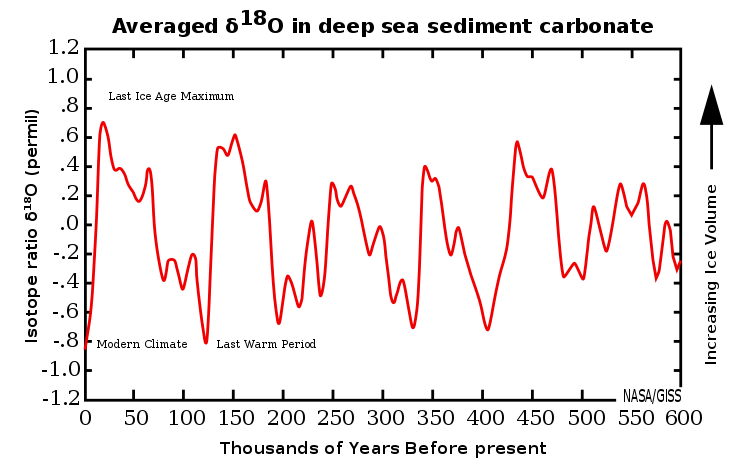
\includegraphics[width=0.9\linewidth]{figures/evol18Osur600kA}
	\caption{Evolution de la présence de $^{18}$O dans les sédiments marins durant les derniers 600\,kA. %La quantité $\delta^{18}$O est un indicateur du volume de glace sur Terre et 
		Son évolution montre une variabilité de 100\,kA dans le climat Terrestre. Image tirée de \cite{giss}.}
	\label{fig:evol18Osur600kA}
\end{figure}

%% https://en.wikipedia.org/wiki/Mid-Pleistocene_Transition
%\begin{figure}
%	\centering
%	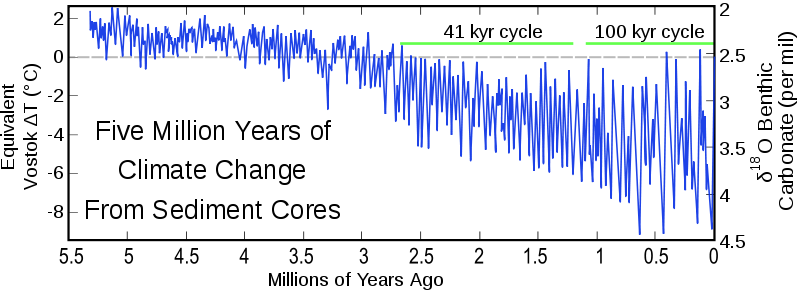
\includegraphics[width=0.9\linewidth]{figures/evol18Osur5MA}
%	\caption{Evolution de la présence de $^{18}$O dans les sédiments marins durant les derniers 5\,MA. Nous observons une variabilité de 41\,kA de 2.6\,MA à 0.9\,MA puis de 100\,kA de 0.9\,MA à nos jours.}
%	\label{fig:evol18Osur5MA}
%\end{figure}
%\todo{fig:cite lisiecki 2005 et wiki mpt}

\begin{figure}
	\centering
	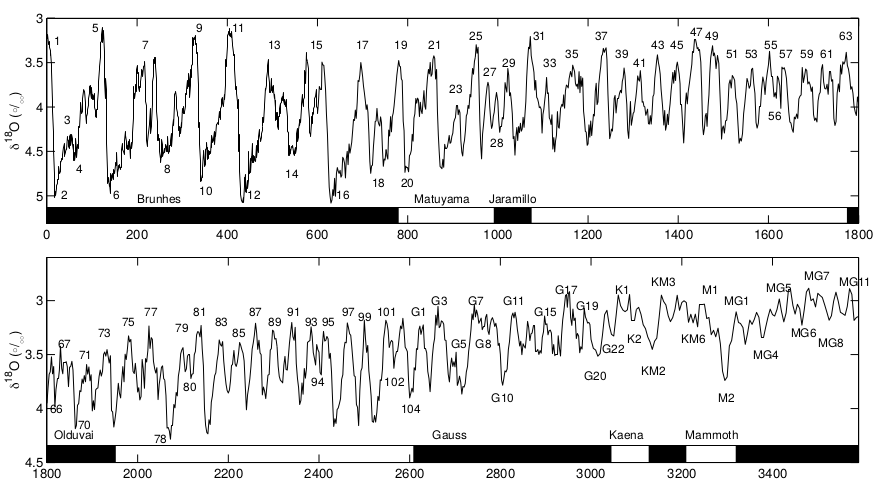
\includegraphics[width=\linewidth]{figures/evol18Osur5MAlisiecki2005}
	\caption{Evolution de la présence de $^{18}$O dans les sédiment marins durant les derniers 5\,MA. Nous observons une variabilité de 41\,kA de 2.6\,MA à 0.9\,MA puis de 100\,kA de 0.9\,MA à nos jours. Image tirée de \cite{lisiecki2005}.}
	\label{fig:evol18Osur5MAlisiecki2005}
\end{figure}



\paragraph{} Les climats passés sont connus à partir de forages, dans de la glace ou des sédiments marins. Plusieurs techniques existent se basant sur la mesure de quantités nous révélant une information sur l'état de la Terre dans le passé. Ces indicateurs peuvent être directs, comme la mesure de la concentration de CO$_2$ dans les carottes de glace, ou indirecte comme la mesure d'abondance relative d'isotopes. La technique la plus fréquente que nous avons rencontré dans ce travail se base sur l'abondance relative des isotopes $^{16}$O et $^{18}$O de l'oxygène dans des sédiments marins de différents types. L'indicateur est défini à partir des mesures d'isotopes selon la formule suivante (voir \cite{wiki_d18O}) 

\begin{equation}\label{d18O}
	\delta^{18}\text{O} = 
	\frac
	{\left(\frac{^{18}\text{O}}{^{16}\text{O}}\right)_{\text{sample}}}
	{\left(\frac{^{18}\text{O}}{^{16}\text{O}}\right)_{\text{standard}}}
	-1 
\end{equation}
et est utilisé pour reconstruire la température de l'environnement dans lequel l'échan- tillon s'est formé ainsi que le volume de glace présent sur les calottes durant les glaciations.

\paragraph{} La figure \ref{fig:evol18Osur600kA} nous renseigne sur l'évolution du climat terrestre durant les derniers 600\,kA \cite{schmidt1999}. Ces données montrent la variation quasi-périodique de la taille des calottes de glace, sur un cycle d'environ 100\,kA. L'évolution sur un temps plus long est donnée sur la figure \ref{fig:evol18Osur5MAlisiecki2005}, basée sur une reconstruction venant de plusieurs sites de forage \cite{lisiecki2005}. Sur cette image, nous pouvons voir une transition dans la périodicité des changement climatique \cite{wiki_mid_pleistocene_transition} \cite{huggett} . Elle se produit il y a environ 900\,kA, au milieu du pléistocène. Les cycles passent d'environ 40\,kA à 100\,kA et augmentent en amplitude. 


\section{Les cycles de Milankovitch}

%% Contenu:  Expliquer ce que c'est, graphes 
%            Référencer les articles originaux si possible
%            ...?

%% SECTION: CYCLES DE MILANKOVITCH

\paragraph{} Les variations du flux de chaleur solaire dans la théorie de Milankovitch sont dû à des cycles dans les paramètres de la trajectoire de la Terre. Les paramètres considérés par Milankovitch sont l'obliquité, l'excentricité et la précession axiale. L'obliquité $\varepsilon$ est l'angle entre l'axe de rotation Terrestre et la normale au plan orbital. L'excentricité $e$ est une mesure du caractère elliptique de la trajectoire et est reliée au grand et petit demi-axes de l'ellipse, respectivement $a$ et $b$, par la formule

\begin{equation}
	e = \sqrt{1-\frac{b^2}{a^2}}.
\end{equation}
Enfin, la précession axiale est la rotation de l'axe de rotation par rapport au repère fixe des étoiles. Le paramètre suivi dans le cas de la précession est le sinus de l'angle $\bar\omega$ décrivant l'état de l'axe dans sa rotation. La figure \ref{fig:MilankovitchCyclesOrbitandCores} reprend l'évolution de ces paramètres orbitaux sur environ 800\,kA avant et après l'instant présent.

\begin{figure}[t]
	\centering
	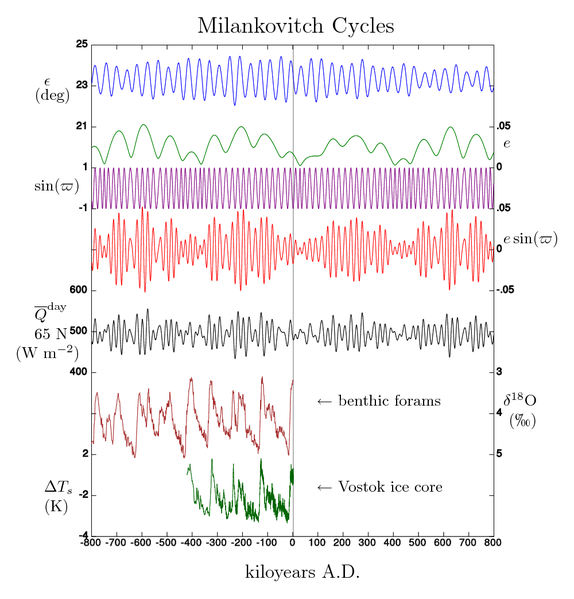
\includegraphics[width=0.9\linewidth]{figures/MilankovitchCyclesOrbitandCores}
	\caption{Cycles de Milankovitch: évolution des paramètres orbitaux. Image tirée de \cite{wiki_milankovitch_cycles}.}
	\label{fig:MilankovitchCyclesOrbitandCores}
\end{figure}

\paragraph{} Le cycle décrit par l'obliquité a une période principale de 41\,kA, i.e. principal pic dans la décomposition spectrale. Il est communément tenu pour responsable de la variation du climat durant le début du pléistocène (2.6\,MA à 0.9\,MA), période durant laquelle le rythme des glaciations suit le cycle d'obliquité de manière assez li
néaire \cite{huggett}. Le cycle décrit par l'excentricité a des pics à 95,125 et environ 400\,kA. Les deux premiers pics, se combinant à environ 100\,kA, sont des candidats pour expliquer l'écart de 100\,kA entre les glaciations plus récentes. Le cycle de précession se compose quant à lui de signaux de 19 et 23\,kA \cite{huggett} \cite{wiki_milankovitch_cycles}.

\paragraph{} Un autre cycle, écarté par Milankovitch pour ne pas avoir d'influence directe sur le flux solaire, est celui de l'inclinaison du plan orbital de la Terre par rapport au repère fixe des étoiles. Celui-ci a une période principale de 100\,kA et intervient ainsi dans certains modèles pour expliquer les dernières glaciations \cite{muller1995}.


\section{Lien entre les cycles de Milankovitch et les \\glaciations}

%% Contenu:  Overview des Modèles/Mécanisme et 
%             leurs problèmes (propres ou commun à la théo Milankovitck),
%            

%% SECTION: LIEN ENTRE LES CYCLES DE MILANKOVITCH ET LES GLACIATIONS

%% PRINCIPAUX PBLMS
% 100ky problem
% pblm transition
% pblm causalité


%% MECANISMES
% Role de l'excentricité 
%  pblm: 1. too weak,  2. main component at 400ky and we see nothing
% Resonance climatique -> rés.stoch. solve the small amplitude pblm (1)
% Role de l'inclinaison orbitale
% Accumulation de glace sur plusieurs cycles court
% Fluctuations venant du soleil
% Couplages avec CO2 et courants océaniques (collecter réfs)
% ...

%% CRITIQUE
% dernier pblm: taille de l'échantillon et stochasticité
% bcp d'effets et corrél sur petit nbre, difficile d'extraire cause-csq
% bien que bcp de pblm, il y a consensus mais on a pas le mécanisme

%% ALTERNATIVES A MILANKOVITCH ?

\paragraph{} Les corrélations entre les données sur l'évolution du climat pendant la période quaternaire et les cycles de Milankovitch durant cette même période semblent indiquer une relation de cause à effet entre ces deux phénomènes 
\footnote{Corrélation n'implique pas causalité, mais il est difficile d'imaginer que le climat puisse influencer la trajectoire Terrestre ou qu'une cause externe et des effets à la fois sur le climat et sur la trajectoire de la Terre. %Nous savons que les cycles observés dans la trajectoire de la Terre sont causés par l'influence des autres planètes majeurs du système solaire. 
Les seule possibilités restantes sont que les corrélations viennent d'un effet de l'orbite sur le climat ou qu'elles sont dues au hasard.}.
Plusieurs problèmes se confrontent cependant à la théorie de Milankovitch, principalement associés à la seconde moitié du pléistocène \cite{wiki_milankovitch_cycles} \cite{huggett}. Pour commencer, le lien entre les variations de 40\,kA que semble suivre les glaciations du début du pléistocène et le cycle de l'obliquité ne tient plus dans le dernier million d'années. Aucun modèle n'a réussi à s'imposer pour expliquer les variations de 100\,kA de cette période \cite{wiki_100ky_problem}. Une des difficultés présentée par ces oscillations réside dans la non-linéarité de la réponse au forçage, contrairement aux oscillations avant la transition. Ensuite, peu d'explications on pu être apportées pour expliquer la transition entre ces deux régimes. Un seul modèle récent a pu reproduire cette transition dans un modèle numérique tentant compte de l'évolution du taux de CO$_2$ et de l'érosion des sols par la calotte de glace \cite{willeit2019}. Enfin, la causalité du phénomène peut parfois être remise en question, comme lors du réchauffement s'étant produit il y a 135\,kA, qui précède l'augmentation du flux solaire d'environ 10\,kA \cite{karner2000}.

\paragraph{} Les périodicités de 100\,kA du dernier million d'années sont souvent attribuées au cycle de l'excentricité, du fait de la proximité avec ses deux composantes à 95 et 125\,kA. Toutefois, cela pose deux problèmes. Le premier est que ce cycle a une composante importante à 400\,kA, qui n'est pas visible dans les variations climatiques. Le second est que les variations du flux solaire causée par le cycle d'excentricité sont beaucoup plus faible que celles provoquées par les cycles d'obliquité et de précession axiale, d'environ 1\%-2\% \cite{ruddiman2006}.

\paragraph{} Un mécanisme qui peut expliquer à la fois l'influence d'une fréquence particulière du forçage et le problème de la petite amplitude présenté au paragraphe précédent réside dans la notion de résonance. Une sensibilité de la dynamique Terrestre à des fréquences de forçage particulières expliquerait comment un cycle spécifique peut régir le climat de la Terre, son effet étant amplifié par la résonance. Le mécanisme de résonance stochastique que nous approfondissons plus loin est un exemple de tel phénomène. 

\paragraph{} Il est également possible que les oscillations de 100\,kA ne sont pas dues aux cycles de l'excentricité. Des explications alternatives existent. En particulier, une hypothèse d'effet indirect a été proposé \cite{muller1995} à travers les variations de l'inclinaison orbitale. L'inclinaison orbitale ne change pas directement le flux solaire mais, en changeant sa course, la Terre pourrait passer dans des nuages de poussières qui affecteraient ensuite le climat. Cette théorie a l'avantage de ne pas présenter le problème de causalité subit par les autres cycles.

\paragraph{} D'autres explications reprennent les cycles de l'obliquité et de la précession axiale ainsi qu'à des effets amplificateurs comme par les gaz à effet de serre. Une hypothèse est que les terminaisons des glaciations de la deuxième moitié du pléistocène ne se produisent plus à chaque cycle. À la place, la glace ne fondrait plus totalement et s'accumulerait progressivement pour ensuite fondre rapidement à des multiples de la période du cycle d'obliquité, dû à une réponse amplifiée par la présence de CO$_2$ \cite{ruddiman2006}. Un tel modèle donne des réchauffement espacés d'environ 80 ou 120\,kA, ce qui semble assez bien décrire l'évolution du climat à cette période. De plus, la transition du milieu du pléistocène s'expliquerait par le changement entre un régime où la fonte de la calotte est totale à chaque cycle et un autre où la fonte est partielle.

\paragraph{} Pour finir, il a été proposé que des variations de l'intensité solaire provenant de l'activité du Soleil même pourraient être à l'origine des cycles de glaciations, via des ondes de diffusions \cite{ehrlich2007}. 

\paragraph{} Malgré toutes ces propositions, le problème posé par les dernières glaciations reste ouvert. Une difficulté importante de cette énigme est la petitesse de l'intervalle de temps en question. Seulement 900\,kA de données sont disponible pour décrire un effet oscillatoire de période 100\,kA, ce qui n'est pas suffisant pour discriminer plusieurs explications concurrentes. La proposition que le climat est contrôlé de manière déterministe par les forçages orbitaux est elle-même fortement discutable et l'on ne peut écarter l'idée que ces oscillations sont principalement le résultat d'un processus stochastique \cite{wunsch2004}.
 
\paragraph{} Au final, en dépit de ses nombreux problèmes, la théorie de Milankovitch fait un consensus assez large dans la communauté scientifique. %\cite{wiki_milankovitch_cycles} \cite{wunsch2004}

\section{Le phénomène de résonance stochastique}

%% Contenu:  Modélisation 0d du climat (Craaford, puis Nicolis et Benzi?),
%            Potentiel climatologique et aspects stochastique (Nicolis),
%            Forçage périodique seul ? (Benzi?),
%            Forçage avec bruit et résonance stochastique (Nicolis) 
%             (Benzi juste pour la résonance stochastique),
%            Mes petits observations supplémentaire sur la résonance
%             et pertinence potentielle ?,
%            Référencer les articles originaux,
%            Illuster avec mes images du code,
%            Présenter code
%            ...?

\subsection{Introduction}

\paragraph{} La résonance stochastique est un phénomène d'amplification de la réponse d'un système à un forçage périodique en présence de bruit. Ce qui caractérise cette résonance est que l'amplification est permise par le bruit agissant sur le système. Ceci est assez contre-intuitif, car généralement la présence de bruit à pour effet de couvrir la réponse au signal en se superposant à ce dernier.

\paragraph{} Un système élémentaire présentant un effet de résonance stochastique est celui constitué d'une particule dans un potentiel en double puits \cite{scholarpedia} -- voir figure \ref{fig:potentiel_double_puits}. La particule effectue naturellement des transitions d'un puits à l'autre à cause du bruit, mais lorsque le taux de ces transitions devient comparable à la fréquence du forçage externe, les transitions se synchronisent avec ce dernier -- voir figure \ref{fig:trajectory_resonant}. Ce phénomène amplifie drastiquement l'effet du forçage, malgré le fait qu'il soit trop petit pour conduire les transitions à lui seul.

\paragraph{} Une explication intuitive de ce mécanisme a été fournie par Benzi \cite{benzi2010} -- voir figure \ref{fig:explication_mecanisme}. L'idée est que le forçage décale périodiquement un puits du potentiel par rapport à l'autre, ce qui a pour effet de rendre les taux de transitions asymétriques et ainsi toujours maintenir la particule dans le puits favorisé par le forçage. 

\begin{figure}[t]
	\centering
	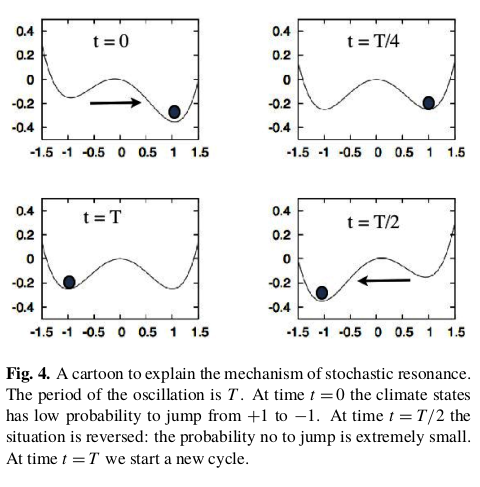
\includegraphics[width=0.8\linewidth]{figures/mecanisme_benzi_2010}
	\caption{Explication du mécanisme de résonance stochastique par R. Benzi. Image tirée de \cite{benzi2010}.}
	\label{fig:explication_mecanisme}
\end{figure}

\subsection{Démonstration analytique}

\paragraph{} Dans cette section, nous allons montrer analytiquement le phénomène de résonance stochastique pour une particule dans un double puits de potentiel. Nous supposons que la dynamique de la particule est sur-amortie. Le forçage prend la forme d'un cosinus %de fréquence $\omega$, de phase $\phi$. L'amplitude du forçage $\epsilon h(x)$ 
dont l'amplitude dépend de la position à travers une fonction $h(x)$. Un paramètre d'expansion $\epsilon \ll 1$ multiplie l'amplitude du forçage afin de le rendre petit par rapport au gradient du potentiel. La présence de bruit s'implémente au travers d'une force stochastique $F(t)$, correspondant à un bruit blanc gaussien vérifiant

\begin{equation}\label{force_stochastique}
\begin{split}
	&\langle F(t) \rangle = 0, \\
	&\langle F(t)F(t') = q^2 \delta(t-t').
\end{split}
\end{equation}
Le paramètre $q^2$ est l'intensité du bruit. L'équation différentielle stochastique décrivant le mouvement de la particule est

\begin{equation}\label{SDE_particule}
	\dv{x}{t} = -\frac{\partial U}{\partial x} + F(t) + \epsilon h(x) \cos(\omega t + \phi)
\end{equation}
De manière équivalente, nous pouvons absorber le forçage dans un potentiel dépendant du temps,

\begin{equation}\label{potentiel_W}
	W(x,t) = U(x) - \epsilon g(x) \cos(\omega t + \phi), \qquad \text{avec } \dv{g}{x}=h.
\end{equation}
Ainsi, l'équation de la dynamique devient

\begin{equation}\label{SDE_potentiel_W}
	\dv{x}{t} = -\frac{\partial W(x,t)}{\partial x} + F(t).
\end{equation}

\paragraph{} En l'absence de forçage, nous sommes en présence d'un processus de diffusion dans le potentiel $U$. Les taux de transition entre les deux puits sont donnés par par formule de Kramers \cite{nicolis1982}:

\begin{equation}\label{Kramers}
	r_\pm = \frac{1}{2\pi} [-U''(x_0)U''(x_\pm)]^{1/2} \exp\left(-\frac{2\Delta U_\pm}{q^2}\right),
\end{equation}
ces taux deviennent rapidement petit lorsque la barrière de potentiel $\Delta U_\pm = U(x_0) - U(x_\pm)$  augmente. Les quantités $x_0, x_-, x_+$ désignent respectivement la position du sommet de la barrière et les minima des puits de part et autre de la barrière. Les probabilités $p_\pm(t)$ pour que la particule se trouve dans les puits obéissent à l'équation maîtresse

\begin{equation}\label{master_sans_forcage}
	\dv{p_\pm(t)}{t} = r_\mp p_\mp(t) - r_\pm p_\pm(t).
\end{equation}
La solution stationnaire est facile à trouver:

\begin{equation}\label{sol_proba_sans_forcage}
	p_\pm = \frac{r_\mp}{r_+ + r_-}, \qquad p_+ + p_- = 1.
\end{equation}

\paragraph{} Pour un petit forçage, les taux sont dépendant du temps et l'équation maîtresse devient

\begin{equation}\label{master_forcage}
	\dv{p_\pm(t)}{t} = r_\mp(t) p_\mp(t) - r_\pm(t) p_\pm(t).
\end{equation}
Nous allons résoudre cette équation de manière perturbative en développant par rapport au paramètre $\epsilon$:

\begin{equation}\label{developpements_perturbatifs}
\begin{split}
	r_\pm(t) &= r_\pm + \epsilon \rho_\pm \cos(\omega t + \phi) + \mathcal O(\epsilon^2), \\
	p_\pm(t) &= p_\pm + \epsilon \pi_\pm  \cos(\omega t + \varphi) + \mathcal O(\epsilon^2).
\end{split}
\end{equation}
Notons qu'à priori, la phase de la solution de l'équation maîtresse n'est pas identique à celle de la perturbation. Nous verrons par la suite qu'elles sont bien différentes. 

\paragraph{} Le développement perturbatif du potentiel est naturellement

\begin{equation}\label{potentiel_perturbatif}
	W(x,t) = U(x) + \epsilon U_1(x,t), \qquad U_1(x,t) = g(x)\cos(\omega t + \phi).
\end{equation}

\paragraph{} Commençons par calculer les taux de transitions $r_\pm(t)$:

\begin{equation}\label{dev_taux_transitions}
\begin{split}
	r_\pm(t) &= \frac{1}{2\pi} [-W''(x_0)W''(x_\pm)]^{1/2} \exp\left( -\frac{2}{q^2} [\Delta U_\pm + \epsilon \Delta U_{1\,\pm}] \right)\\
	&= \frac{1}{2\pi} [-U''(x_0)U''(x_\pm)]^{1/2} \exp\left( -\frac{2}{q^2} [\Delta U_\pm + \epsilon \Delta U_{1\,\pm}] \right) \left( 1 + \sum_{i=0,\pm} \mathcal O\left( \frac{\epsilon g''(x_i)}{U''(x_i)} \right)  \right)  \\
	&\approx r_\pm \exp\left( -\frac{2\epsilon}{q^2} \Delta U_{1\,\pm} \right)\\
	&= r_\pm \left( 1 - \frac{2\epsilon}{q^2} \Delta U_{1\,\pm} + \mathcal O\left( \frac{\epsilon}{q^2} \Delta U_{1\,\pm} \right)^2 \right) 
\end{split}
\end{equation}
avec $\Delta U_{1\,\pm} = g(x_0)-g(x_\pm)$. Ainsi la perturbation au premier ordre prend la forme
\begin{equation}\label{rho_pm}
	\rho_\pm = - \frac{1}{\pi q^2} [-U''(x_0)U''(x_\pm)]^{1/2} [g(x_0)-g(x_\pm)] \exp\left( - \frac{2}{q^2} \Delta U_\pm \right) 
\end{equation}
Cette expression n'est valable que %si la modulation $g(x)$ de l'amplitude du forçage est faible comparé à la barri 
sous les conditions suivantes:

\begin{equation}\label{conditions_validite_perturbation}
	\epsilon |g(x_0)-g(x_\pm)| \ll q^2 \quad \text{et} \quad \frac{g''(x_i)}{U''(x_i)} \ll \frac{[g(x_0)-g(x_\pm)]}{q^2}.
\end{equation}
La première condition revient à demander à ce que le forçage ne domine pas la dynamique du système, ce qui va de soi pour les situations où la résonance stochastique est d'intérêt. La seconde demande à ce que la variation du forçage en fonction de la position ne soit pas trop importante. Cette dernière condition n'est pas relevante lorsque l'amplitude du forçage est uniforme.

\paragraph{} Ayant obtenu les taux de transitions au premier ordre, nous pouvons remplacer les taux de transitions dans l'équation maîtresse \ref{master_forcage}. À l'ordre zéro, nous retombons naturellement sur la solution sans forçage. Au premier ordre, l'équation maîtresse est un système de deux équations couplées pour les perturbations au premier ordre des probabilités:

\begin{equation}\label{master_premier_ordre_couple}
\begin{split}
	-\pi_\pm \omega \sin(\omega t + \varphi) &= 
	\left[\rho_\mp \frac{r_\pm}{r_+ + r_-} - \rho_\pm \frac{r_\mp}{r_+ + r_-} \right] \cos(\omega t + \phi) \\
	&\ \ + [r_\mp \pi_\mp - r_\pm \pi_\pm] \cos(\omega t + \varphi).
\end{split}
\end{equation}
Ce système ce découple toutefois facilement en invoquant la conservation de la probabilité, $p_+ + p_- = 1$, qui impose $\pi_+ = -\pi_-$. Ainsi,

\begin{equation}\label{master_premier_ordre_decouple}
\begin{split}
	-\pi_\pm \omega \sin(\omega t + \varphi) &= 
	\left[\rho_\mp \frac{r_\pm}{r_+ + r_-} - \rho_\pm \frac{r_\mp}{r_+ + r_-} \right] \cos(\omega t + \phi) \\
	&\ \ - [r_\mp + r_\pm] \pi_\pm \cos(\omega t + \varphi).
\end{split}
\end{equation}
En nommant les quantités entre crochets $A_\pm$ et $B_\pm$, les équations maîtresses se réécrivent

\begin{equation}\label{master_premier_ordre_AB}
	-\pi_\pm \omega \sin(\omega t + \varphi) = 
	A_\pm \cos(\omega t + \phi) - B_\pm \pi_\pm \cos(\omega t + \varphi).
\end{equation}
L'une d'entre elles est maintenant redondante.

\paragraph{} Pour résoudre l'équation maîtresse au premier ordre, nous allons utiliser le fait que cette équation reste valide en tout instant pour la projeter sur la base formée par $\sin(\omega t+\phi)$ et $\cos(\omega t+\phi)$. Nous commençons pour mettre en évidence ces deux quantités en séparant l'angle $\varphi = \phi + \Delta \phi$:

\begin{equation}
\begin{split}
	&-\pi_+ \omega [\sin(\omega t+\phi)\cos(\Delta\phi) + \cos(\omega t+\phi)\sin(\Delta\phi)] \\
	&= A_+ \cos(\omega t+\phi) - B_+ \pi_+ [\cos(\omega t+\phi)\cos(\Delta\phi) - \sin(\omega t+\phi)\sin(\Delta\phi)].
\end{split}
\end{equation}
L'équation en sinus donne le décalage de phase $\Delta\phi$:

\begin{equation}\label{eq_sinus}
	\pi_+ \omega \cos(\Delta\phi) = -B_+ \sin(\Delta\phi) \iff \tan(\Delta\phi) = -\frac{\omega}{r_+ + r_-}.
\end{equation}
L'équation en cosinus permet ensuite de trouver l'amplitude de la perturbation sur la probabilité:

\begin{equation}\label{eq_cosinus}
\begin{split}
	-\pi_+\omega \sin(\Delta\phi) &= A_+ - B_+ \pi_+ \cos(\Delta\phi) \\
	-\pi_+ \omega \frac{-\omega/B_+}{\sqrt{1+\omega^2/B_+^2}} &= A_+ - B_+ \pi_+ \frac{1}{\sqrt{1+\omega^2/B_+^2}} \\
	\pi_+ (\omega^2 + B_+^2) &= A_+B_+ \sqrt{1+\omega^2/B_+^2}
\end{split}
\end{equation}
Ainsi,

\begin{equation}\label{expr_pi_AB}
	\pi_+ = \frac{A_+}{B_+}  \frac{1}{\sqrt{1+\omega^2/B_+^2}} = \frac{A_+}{B_+} \frac{1}{\sqrt{1+\omega^2/(r_+ + r_-)^2}}
	%\frac{r_+ + r_-}{(r_+ + r_-)^2+\omega^2}
	.
\end{equation}

\paragraph{} Le calcul du rapport $A_+/B_+$ se fait en insérant les expression des taux de transitions aux ordres zéro et un. Nous obtenons

\begin{equation}\label{rapport_AB}
\begin{split}
	\frac{A_+}{B_+} &= \frac{\rho_- r_+}{(r_+ + r_-)^2} - \frac{\rho_+ r_-}{(r_+ + r_-)^2} \\
	&= \frac{2}{q^2} [g(x_-)-g(x_+)] 
	\frac{
		[U''_{0-}U''_{0+}]^{1/2} \exp(-\frac{2}{q^2} (\Delta U_+ + \Delta U_-))
	}
	{
		\left[
			[U''_{0+}]^{1/2} \exp(-\frac{2}{q^2} \Delta U_+) + [U''_{0-}]^{1/2} \exp(-\frac{2}{q^2} \Delta U_-)
		\right]^2
	} ,
\end{split}
\end{equation}
où $U''_{0\pm} = -U''(x_0)U''(x_\pm)$. Nous avons maintenant résolu l'équation maîtresse \ref{master_premier_ordre_AB} et avons calculé la réponse du système bruité à un forçage extérieur.

\paragraph{} La première chose que nous pouvons noter est le facteur $1/\sqrt{1+\omega^2/(r_+ + r_-)^2}$ dans l'expression de la réponse $\pi_+$. Le phénomène de résonance est bien visible lorsque la fréquence du signal $\omega$ approche la fréquence résonante $\omega_r = r_+ + r_-$. Notons que la réponse est fortement amortie pour les basses fréquences mais est encore assez grande dans la limite de basse fréquences. Comme l'a souligné Nicolis, cette propriété rend le qualificatif de "résonance" discutable \cite{nicolis1982}. Le système bruité se comporte un peu comme un filtre passe-bas.

\paragraph{} Remarquons aussi que la réponse est pratiquement nulle si les deux puits du potentiel sont à des hauteurs trop différentes. Plus précisément, si $|\Delta U_+ - \Delta U_-| \gg q^2$, alors les taux de transitions sont très inégaux et la particule aura une probabilité quasi nulle de se trouver dans le puits le plus haut.
Schématiquement, si l'on dénote par $e^\pm$ les exponentielles $\exp(-2\Delta U_\pm/q^2)$ et que le puits $x_-$ est le plus stable, la probabilité au premier ordre d'être dans le puits instable se comporte comme

\begin{equation}
	p_+ = \frac{r_-}{r_+ + r_-} \sim \frac{e^-}{e^+ + e^-} \approx \frac{e^-}{e^+} \ll 1.
\end{equation}
De même, la réponse au premier ordre s'annule exponentiellement vite car

\begin{equation}
	\pi_+ \sim \frac{A_+}{B_-} \sim \frac{e^+e^-}{(e^+ + e^-)^2} \approx \frac{e^-}{e^+} \ll 1.
\end{equation}
Pour que le phénomène de résonance puisse jouer un rôle, il est donc nécessaire que le système présente deux états de pareille stabilité. Dans le cadre de systèmes climatiques, Nicolis fait référence à un état de coexistence entre deux climats \cite{nicolis1981} \cite{nicolis1982}. Dans le cas d'un potentiel présentant un axe de symétrie entre les deux puits, l'expression de la réponse $\pi_+$ se simplifie en

\begin{equation}\label{pi_sans_exp}
	\pi_+ = \frac{1}{2q^2} \frac{g(x_-) - g(x_+)}{\sqrt{1+\omega^2/(r_+ + r_-)^2}}.
\end{equation}







\subsection{Démonstration numérique}

\paragraph{} Dans cette section, nous nous restreignons au cas d'un potentiel en double puits avec un forçage uniforme, $h(x)=1$.
Nous faisons la simulation numérique de la dynamique stochastique \ref{SDE_particule} et confronterons les résultats aux expressions analytiques de la section précédente. La simulation numérique a l'avantage de nous permettre de sortir des limites de validité des approximations faites dans la partie analytique et d'étendre ainsi l'exploration du phénomène.


\subsubsection{Cas d'un double puits de potentiel}

Le potentiel considéré -- voir figure \ref{fig:potentiel_double_puits} -- est donné par

\begin{equation}\label{potentiel_double_puits}
U(x) = -\frac{\lambda}{2}x^2 + \frac{1}{4} x^4, \qquad \lambda>0.
\end{equation}
les minimas sont $x_\pm = \pm \lambda^{1/2}$ et sont séparés par une barrière de potentiel en $x=0$ d'une hauteur $\Delta U_\pm = \lambda^2/4$. Les taux de transitions en l'absence de forçage valent

\begin{equation}\label{r_dbpuits}
	r = r_\pm = \frac{\lambda}{\sqrt 2\pi} \exp\left( -\frac{\lambda^2}{2 q^2} \right) 
\end{equation}
et l'amplitude de la réponse $p_+(t) = p_+ + A\cos(\omega t+\varphi)$ à un petit forçage est

\begin{equation}\label{pi_dbpuits}
	|A| = |\epsilon \pi_+| = \frac{\epsilon}{q^2} \frac{\lambda^{1/2}}{\sqrt{1+\omega^2/(2r)^2}}.
\end{equation}

%Le décalage de phase vaut quant à lui $\Delta\phi = \arctan(-\omega/(2r))$.

\begin{figure}
	\centering
	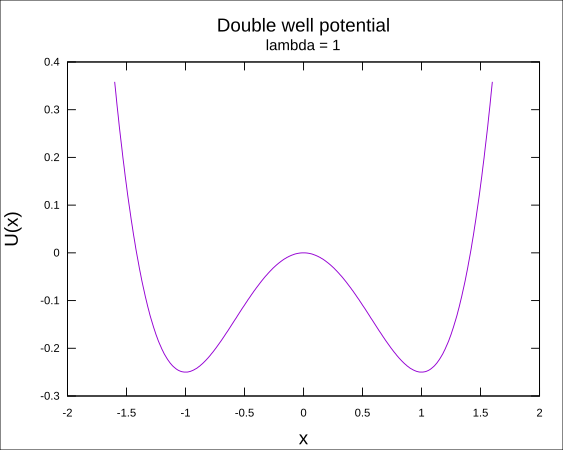
\includegraphics[width=0.8\linewidth]{figures/potential}
	\caption{Potentiel en double puits utilisé pour l'application numérique.}
	\label{fig:potentiel_double_puits}
\end{figure}


\subsubsection{Simulation du processus stochastique}

\paragraph{} La dynamique stochastique \ref{SDE_particule} s'intègre en discrétisant le temps en pas $dt$. L'équation discrétisée devient

\begin{equation}\label{SDE_discrete}
	x_{n+1} = \frac{\partial U(x_n)}{\partial x} dt + \epsilon h(x_n) \cos(\omega t + \phi) dt + \sqrt{q^2 dt} \,G_n,
\end{equation}
où la variable $G_n$ est une variable aléatoire suivant une distribution normale avec 

\begin{equation}\label{G_n}
\begin{split}
	&\langle G_n \rangle = 0,\\
	&\langle G_nG_{n'} \rangle = \delta_{nn'}.
\end{split}
\end{equation}

\paragraph{} Dans les limites de validité du développement de la section précédente, ici $\epsilon \ll q^2 \lambda^{-1/2}$, la simulation du processus pour le potentiel en double puits montre des transitions aléatoires entre les puits -- voir figure \ref{fig:trajectory_random}. Ceci est dû au fait que la réponse est trop petite pour être vue sur le graphique de la trajectoire. Dans la section suivante, nous allons intégrer sur des temps plus long et prendre la transformée de Fourier du signal afin d'extraire la réponse au premier ordre. Contrairement au développement perturbatif de la théorie, la simulation nous permet d'analyser la réponse non-linéaire du système pour de plus grands forçages. La figure \ref{fig:trajectory_resonant} montre un exemple de synchronisation de la trajectoire avec le forçage. Bien que le forçage soit assez grand pour causer des effets non-linéaires, la synchronisation est bien causée par le bruit dans le système. La trajectoire déterministe pour un même forçage ne donne pas de telle transitions, la réponse déterministe étant bien trop petite -- voir figure \ref{fig:trajectory_deterministic_small}.


\begin{figure}[p]
	\centering
	
	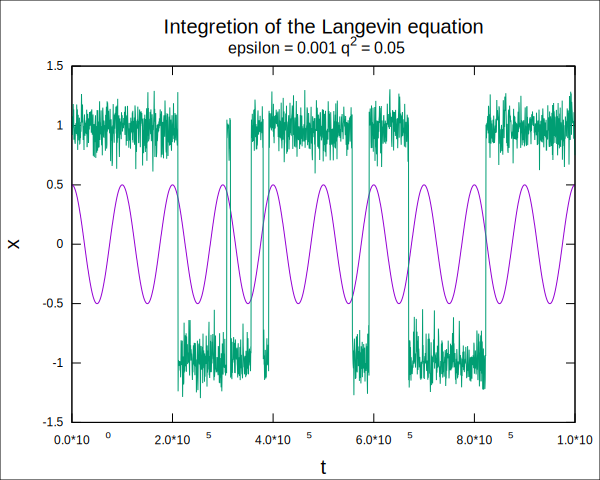
\includegraphics[width=0.8\linewidth]{figures/trajectory_random}
	\caption{Trajectoire pour un petit forçage. La réponse $\pi_+$ est linéaire et beaucoup plus petite que la probabilité à l'ordre zéro. Les transitions sont donc encore aléatoires. L'amplitude du forçage (en mauve) est ajustée pour des raisons de visibilité.}
	\label{fig:trajectory_random}
	
	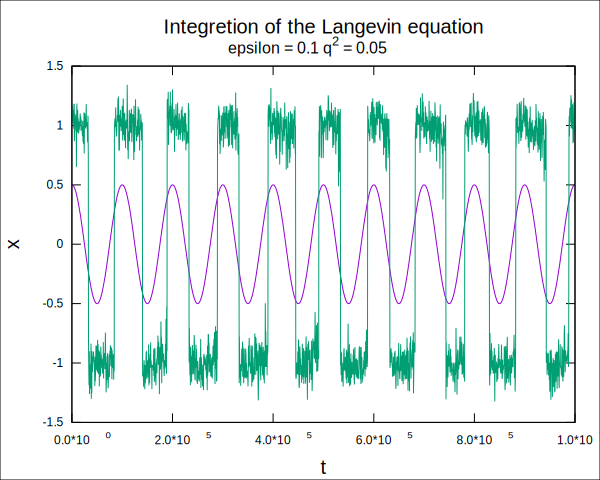
\includegraphics[width=0.8\linewidth]{figures/trajectory_resonant}
	\caption{Trajectoire pour un forçage d'amplitude comparable à $q^2$. La réponse $\pi_+$ est non-linéaire et efface le comportement à l'ordre zéro. Les transitions sont synchronisées avec le forçage. Le décalage de phase est très net sur cette image. L'amplitude du forçage (en mauve) est ajustée pour des raisons de visibilité.}
	\label{fig:trajectory_resonant}
\end{figure}

\begin{figure}[p]
	\centering
	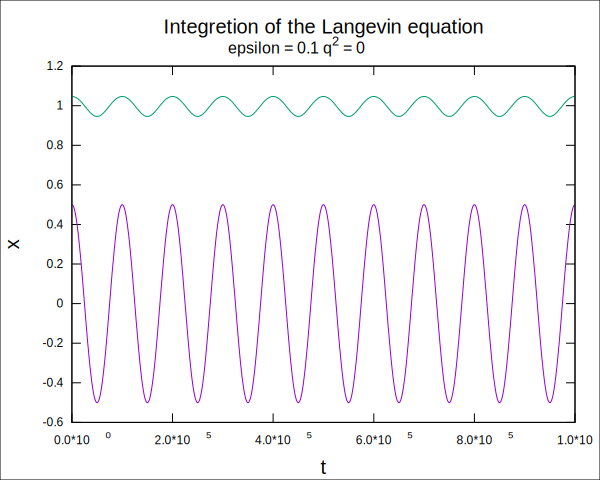
\includegraphics[width=0.8\linewidth]{figures/trajectory_deterministic_small}
	\caption{Réponse déterministe au forçage externe. Cette image montre que la synchronisation observée pour $\epsilon = 0.1$ -- voir figure \ref{fig:trajectory_resonant} -- est bien due au mécanisme de résonance stochastique. L'amplitude du forçage (en mauve) est ajustée pour des raisons de visibilité.}
	\label{fig:trajectory_deterministic_small}

	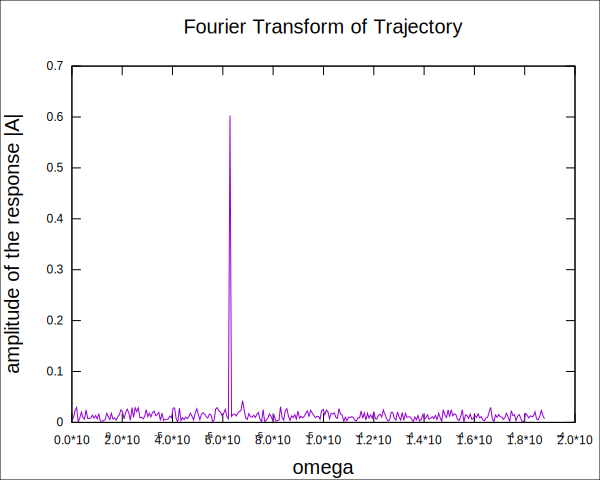
\includegraphics[width=0.8\linewidth]{figures/spectrum_resonant}
	\caption{Transformée de Fourier de la trajectoire résonante de la figure \ref{fig:trajectory_resonant}.}
	\label{fig:spectrum_resonant}
\end{figure}

\subsubsection{Analyse de Fourier et amplification en fonction du bruit}

\begin{figure}
	\centering
	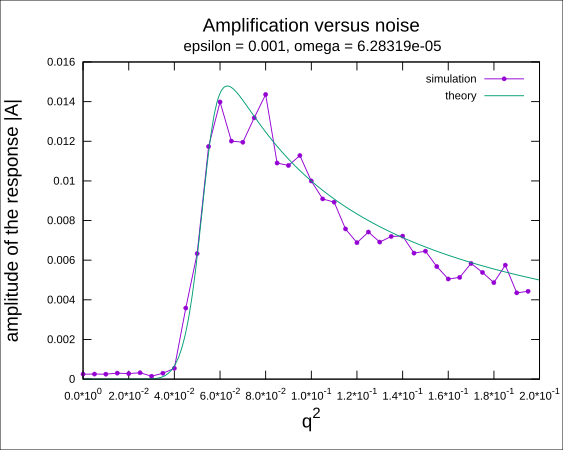
\includegraphics[width=0.8\linewidth]{figures/amplification_versus_noise}
	\caption{Amplitude de la réponse linéaire à un petit forçage en fonction de l'intensité du bruit. Nous pouvons clairement observer le phénomène de résonance stochastique dû à la présence de bruit dans le système.}
	\label{fig:amplification_versus_noise}
\end{figure}

\paragraph{} Pour pouvoir comparer les prévisions analytiques avec la simulation numérique, il faut pouvoir extraire l'amplitude de la réponse au premier ordre. Nous réalisons cela en intégrant le système sur un temps assez long pour avoir une résolution assez bonne sur la probabilité de résidence en chaque puits à l'ordre $\epsilon$ et prenons ensuite la transformée de Fourier de la trajectoire. Nous sommes intéressés par le coefficient de Fourier associé à la fréquence du signal.

\paragraph{} Numériquement, nous faisons une transformée de Fourier discrète des positions $\{f_j\}_{j=0}^N$ enregistrés à intervalle régulier depuis la trajectoire $f(t)$. L'expression des valeurs discrétisées de la  transformée de Fourier est 

\begin{equation}\label{f_hat_k}
	\hat f_k = \frac{1}{\sqrt{2\pi}} \sum_{j=0}^{N} \Delta t f_j e^{-i\omega t}.
\end{equation}
Les temps et fréquences sont discrétisés de sorte à ce que $t=j\Delta t$ et $\omega = k\Delta \omega$. L'intervalle des fréquences est relié à l'intervalle temporel par $\Delta \omega = 2\pi/(N\Delta t)$. De cette manière, nous pouvons réaliser la transformée de Fourier d'une trajectoire, comme par exemple la trajectoire résonante $\epsilon=0.1$ -- voir figures \ref{fig:trajectory_resonant} et \ref{fig:spectrum_resonant}.

\paragraph{} Pour retrouver l'amplitude de la réponse à un petit forçage, nous analysons comment un signal $A\cos(\omega_0 t)$ se transforme avec \ref{f_hat_k} et déduisons que l'amplitude $A$ se retrouve avec la relation $|A| = |\hat f_k|\Delta \omega/\sqrt{2\pi}$, en utilisant la fréquence $\omega_0=k\Delta\omega$ du signal. Ainsi, nous pouvons nous servir de la simulation pour observer comment l'amplitude de la réponse varie avec l'intensité du bruit. La figure \ref{fig:amplification_versus_noise} montre ces résultats en parallèle avec la prédiction théorique.
Il est clair de cette observation que l'amplification du signal résonne avec une intensité critique du bruit, en dessous de laquelle la réponse est pratiquement nulle.

\subsection{Intérêt pour la compréhension des glaciations du quaternaire}

\paragraph{} Comme nous l'avons déjà souligné plus haut, un tel mécanisme d'amplification de petits forçage présente un certain attrait pour la théorie de Milankovitch. En effet, le problème des glaciations de la fin du quaternaire, espacées de 100\,kA, est que le principal cycle orbital candidat est celui de l'excentricité dont les composantes à 100\,kA ne font varier que peu le flux solaire (environ 0.1\% \cite{scholarpedia}). Le phénomène de résonance stochastique pourrait donc expliquer comment ce signal serait capable d'influencer le climat Terrestre. 

\paragraph{} Dans leurs articles du début des années 1980, Nicolis et Benzi étudient la variabilité du climat à travers ce qui appellent un potentiel climatique \cite{nicolis1982} \cite{benzi1983}. Cette grandeur joue le rôle du potentiel que ressent la particule dans nos dérivations ci-dessus. Le système étudié est dans ce cas-ci le climat Terrestre et son espace de configurations n'a qu'une seule variable, la température moyenne de la Terre\footnote{On parle de modèle zéro-dimensionnel lorsqu'aucune variable spatiale décrit le système.}. La dérivation d'un tel potentiel se fait à partir d'un bilan énergétique de la Terre (modèles dits de Budyko-Sellers). Les apports d'énergie sont le flux solaire et les pertes sont le rayonnement infrarouge ainsi que la réflexion des rayons solaires par la glace. L'équation bilan obtenue est du type

\begin{equation}\label{bilan_thermique}
	c\dv{T}{t} = R_{in}(T) - R_{out}(T) = Q_0(1-\alpha(T)) + \varepsilon \sigma T^4,
\end{equation}
où $c$ est la capacité calorifique de la Terre, $Q_0$ est le flux solaire moyen, $\alpha(T)$ l'albédo de la Terre en fonction de la température, $\varepsilon$ l'émissivité de la Terre et $\sigma$ la constante de Stefan.
         
\paragraph{} Dans son article, Nicolis utilise un modèle linéaire par morceaux pour la fonction albédo $\alpha(T)$ -- voir figure \ref{fig:bilan_thermique_albedo_lineaire}. La conclusion
\footnote{Sur une note personnelle: Comme expliqué dans l'article (\cite{nicolis1982}), le modèle utilisée pour la fonction albédo mène à des climats stables pour une Terre entièrement couverte de glace ainsi que le climat actuel. Il semble donc que ce modèle doit être encore raffiné pour expliquer les glaciations récentes, qui n'étaient que partielles.}
de son analyse est qu'on arrive à reproduire une résonance pour le cycle de 100\,kA. Du côté du groupe de Benzi, la fonction albédo est approximée par une forme présentant le double puits par construction et les paramètres sont ensuite ajustés pour que le modèle soit cohérent avec des résultats connus. Ce dernier groupe arrive aussi à la conclusion qu'une amplification par résonance stochastique est possible pour des valeurs de paramètres semblable à ceux du climat Terrestre. 

\paragraph{} Pour finir, malgré l'attrait que peut présenter le phénomène de résonance stochastique, il ne semble pas que de travaux plus récents ait permit de réserver un rôle essentiel au mécanisme pour faire le lien entre les cycles de Milankovitch et les glaciations quaternaires. Toutefois, une explication solide à ce lien est encore recherchée à ce jour. 

\begin{figure}
	\centering
	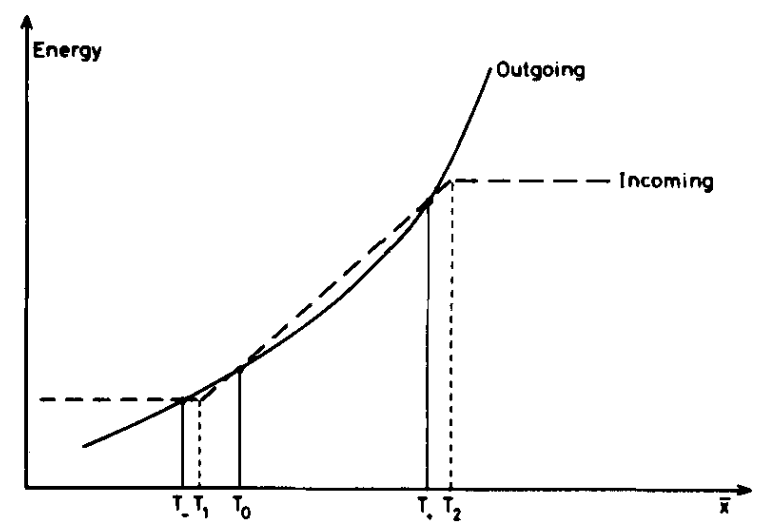
\includegraphics[width=0.8\linewidth]{figures/bilan_thermique_albedo_lineaire}
	\caption{Bilan énergétique suivant le modèle d'albédo linéaire par morceaux employé par Nicolis \cite{nicolis1982}. Image tirée de l'article.}
	\label{fig:bilan_thermique_albedo_lineaire}
\end{figure}









%%%%%%%%%%%%%%%%%%%%%%

%\section{Conclusions}

%% Contenu:  ... résumer le travail ...
%            Dire que ce n'est pas settled (pas l'air en tout cas)

%\input{inputs/conclusions}


%%%%%%%%%%%%%%%%%%%%%%%%%%%%%%%%%%%%%%%%%%%%%%%%%%%%%%%%%%%%%%%%%%

\newpage
\printbibliography

\end{document} 
